\documentclass[xcolor=pdftex,dvipsnames,table]{beamer}
\usetheme{Darmstadt}
\usepackage{etex}
\providecommand\thispdfpagelabel[1]{}
\usepackage{amsmath}
\usepackage{amssymb}
\usepackage{amsthm}
\usepackage{listings}
\usepackage{graphics}
\usepackage{framed}
\usepackage{etex}
\usepackage[all]{xy}
\usepackage{svg}
\usepackage{xspace,listings,ulem,tikz}
\usepackage[outline]{contour}
\usepackage[absolute,overlay]{textpos}
\usepackage{hhline}
\usepackage{pgffor}
\usepackage[square,sort,comma,numbers]{natbib}
\usepackage{CJKutf8}
\setbeamertemplate{footline}[frame number]
\tikzset{
    onslide/.code args={<#1>#2}{% http://tex.stackexchange.com/a/6155/16595
        \only<#1>{\pgfkeysalso{#2}}
    },
    hideshow/.style args={<#1><#2>#3}{%
        onslide=<#1>{move to},
        onslide=<#2>{#3}
    }
}
\lstset{
         basicstyle=\footnotesize\ttfamily, % Standardschrift
         %numbers=left,               % Ort der Zeilennummern
         numberstyle=\tiny,          % Stil der Zeilennummern
         %stepnumber=2,               % Abstand zwischen den Zeilennummern
         numbersep=5pt,              % Abstand der Nummern zum Text
         tabsize=2,                  % Groesse von Tabs
         extendedchars=true,         %
         breaklines=true,            % Zeilen werden Umgebrochen
         keywordstyle=\color{red},
 %        keywordstyle=[1]\textbf,    % Stil der Keywords
 %        keywordstyle=[2]\textbf,    %
 %        keywordstyle=[3]\textbf,    %
 %        keywordstyle=[4]\textbf,   \sqrt{\sqrt{}} %
         %stringstyle=\color{white}\ttfamily, % Farbe der String
         showspaces=false,           % Leerzeichen anzeigen ?
         showtabs=false,             % Tabs anzeigen ?
         xleftmargin=3pt,
         framexleftmargin=3pt,
         framexrightmargin=1pt,
         framexbottommargin=3pt,
         language=C++,
         %backgroundcolor=\color{lightgray},
         showstringspaces=false      % Leerzeichen in Strings anzeigen ?        
 }

 \usetikzlibrary{arrows}
 \usepackage{caption}
\DeclareCaptionFont{white}{\color{white}}
\DeclareCaptionFormat{listing}{\colorbox[cmyk]{0.43, 0.35, 0.35,0.01}{\parbox{\textwidth}{\hspace{15pt}#1#2#3}}}
\captionsetup[lstlisting]{format=listing,labelfont=white,textfont=white, singlelinecheck=false, margin=0pt, font={bf,footnotesize}}
\beamertemplatenavigationsymbolsempty
\newcommand{\N}{\ensuremath{\mathbb{N}}} 
\newcommand{\R}{\ensuremath{\mathbb{R}}} 
\newcommand{\RR}{\ensuremath{\mathbb{R}}} 
\newcommand{\C}{\ensuremath{\mathbb{C}}} 
\newcommand{\Q}{\ensuremath{\mathbb{Q}}} 
\newcommand{\Z}{\ensuremath{\mathbb{Z}}} 
\newcommand{\D}{\ensuremath{\mathbb{D}}}
\newcommand{\lb}{\mathrm{lb}}
\newcommand{\dy}{\mathrm{dy}}
\newcommand{\cc}{\texttt{C++}\xspace}
\newcommand{\bin}{\mathrm{bin}}
\newcommand{\irram}{\texttt{iRRAM}\xspace}
\newcommand{\code}[1]{\texttt{#1}}
\newcommand{\sharpp}{\ensuremath{\#\mathcal P}\xspace}
\newcommand{\p}{\ensuremath{\mathcal P}\xspace}
\newcommand{\np}{\ensuremath{\mathcal{ NP }}\xspace}
\newcommand{\pspace}{\ensuremath{\mathcal{ PSPACE }}\xspace}
\newcommand{\npc}{\ensuremath{\mathcal{ NP }c}\xspace}
\newcommand{\eXp}{\ensuremath{\mathcal{EXP}}\xspace}
\newcommand{\sharppu}{\ensuremath{\#{\mathcal P}_1}\xspace}
\newcommand{\fp}{\ensuremath{\mathcal{FP}}\xspace}
  \newcommand{\baana}{\code{BA\_ANA}\xspace}
  \newcommand{\anarect}{\code{ANA\_RECT}\xspace}
  \newcommand{\powerseries}{\code{POWERSERIES}\xspace}
  \newcommand{\poly}{\code{POLY}\xspace}
  \newcommand{\func}{\code{FUNC}\xspace}
  \newcommand{\real}{\code{REAL}\xspace}
  \newcommand{\complex}{\code{COMPLEX}\xspace}
	\newcommand{\abs}[1]{\left|#1\right|}
  \newcommand{\temp}{\textcolor{red}}
  \newcommand{\seq}{\mathbf}
\newcommand{\fpu}{\ensuremath{\mathcal{FP}_1}\xspace}
\DeclareMathOperator{\dom}{\mathrm{dom}}
\newtheorem{conjecture}{Conjecture} 
\newtheorem{representation1}{Representation 1} 
\newtheorem{representation1b}{Representation 1'} 
\newtheorem{representation2}{Representation 2} 
\title[data-types for multidimensional functions]{On data-types for multidimensional functions in Exact Real Arithmetic
}
\author[ H. Thies]{
		Holger Thies \footnote{Joint work with Akitoshi Kawamura and Florian Steinberg}
}
\institute[The University of Tokyo]{
  The University of Tokyo
}
\begin{document}
\setbeamercolor{note}{fg=black,bg=lightgray} 
\date{May 9, 2016}
\frame{
\titlepage
}
\section{Real Computability}
\subsection{Computable Reals}
\begin{frame}
  \frametitle{Computers and Real Numbers}
  \begin{itemize}[<+->]
  \item The set of real numbers is uncountable
    \item It is not possible to write every real number as finite string over a finite alphabet
    \item Most common way: represented by a fixed-length string (e.g. floating point)
    \item Can be implemented in hardware, thus very fast
      \item Rounding is necessary
     \item Does not behave well from a mathematical point of view (closure under composition,...) 
       \item Not a safe way to do computations
    \end{itemize}
  \end{frame}
\begin{frame}
\frametitle{Computable Real Numbers}
  A real number is called computable if it can be approximated up to any desired precision.
  \vfill
  \pause
\begin{minipage}{.45\textwidth}
		\begin{figure}
		\centering
    \vfill
		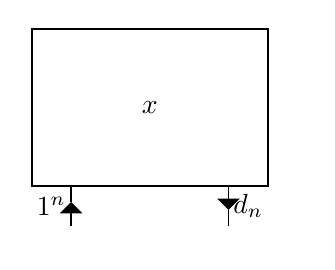
\begin{tikzpicture}
				\path (0,0) rectangle (3.5,-2.7);
			%x
				\draw[thick] (0,0) rectangle (3,-2);
				\node at (1.5,-1) {$x$};
				\draw (.5,-2) -- (.5,-2.2);
				\draw[-triangle 90] (.5,-2.5) -- (.5,-2.2);
				\node at (.25,-2.25) {$1^n$};
				\draw[-triangle 90] (2.5,-2) -- (2.5,-2.3);
				\draw (2.5,-2.3) -- (2.5,-2.5);
				\node at (2.75,-2.25) {$d_n$};
				%\node<4-> at (2.85,-2.25) {$d_{n,i}$};
				%\node<4-> at (1.5,-1) {$(a_i)$};
				%\draw<4-> (1,-2) -- (1,-2.2);
				%\draw<4->[-triangle 90] (1,-2.5) -- (1,-2.2);
				%\node<4-> at (1.25,-2.25) {$1^i$};
		\end{tikzpicture}
		\end{figure}
	\end{minipage}
	\hfill
        \pause
	\begin{minipage}{.45\textwidth}
		\begin{tikzpicture}
			\path (-1.7,1.7) rectangle (3.7,-5.2);
			%x
				\draw<4-> (0,0) rectangle (3,-2);
				\node<4-> at (1.5,-1) {$x$};
				\draw<4-> (1,-2) -- (1,-2.2);
				\draw<4->[-triangle 90] (1,-2.5) -- (1,-2.2);
				\node<4-> at (.5,-2.25) {$1^m$};
				\draw<4->[-triangle 90] (2,-2) -- (2,-2.3);
				\draw<4-> (2,-2.3) -- (2,-2.5);
				\node<4-> at (2.5,-2.25) {$d_m$};
			%f
				\draw[thick] (0,-2.5) rectangle (3,-4.5);
				\node at (1.5,-3.5) {$f$};
				\draw (1,-4.5) -- (1,-4.7);
				\draw[-triangle 90] (1,-5) -- (1,-4.7);
				\node at (.5,-4.75) {$1^n$};
				\draw[-triangle 90] (2,-4.5) -- (2,-4.8);
				\draw (2,-4.8) -- (2,-5);
				\node at (2.5,-4.75) {$d_n$};
			%f(x)
				%\draw (-1.5,.5) rectangle (3.5,-4.5);
				%\node at (-.75,-2) {$f(x)$};
		\end{tikzpicture}
	\end{minipage}
\end{frame}
\subsection{Computable Functions}
\begin{frame}
  \frametitle{Representations}
  A representation for a set $X$ is a partial surjective function $\rho: \Sigma^{**} \to X$.
  \pause
  \vfill
  \begin{minipage}{.37\textwidth}
  \begin{displaymath}
    \xymatrix{
        \Sigma^{**} \ar[r]^F \ar[d]_\alpha & \Sigma^{**} \ar[d]^{\beta} \\
        X \ar[r]_{f}       & Y }
  \end{displaymath} 
  \end{minipage}
  \hfill
  \pause
  \begin{minipage}{.45\textwidth}
    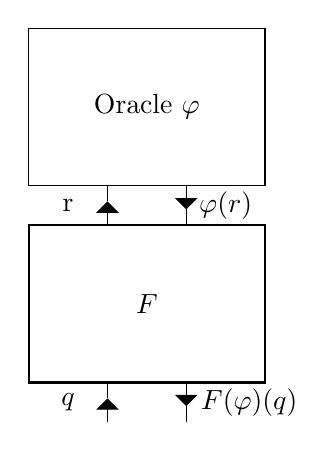
\begin{tikzpicture}
      %x
      \draw (0,0) rectangle (3,-2);
      \node at (1.5,-1) {Oracle $\varphi$};
      \draw (1,-2) -- (1,-2.2);
      \draw[-triangle 90] (1,-2.5) -- (1,-2.2);
      \node at (.5,-2.25) {r};
      \draw[-triangle 90] (2,-2) -- (2,-2.3);
      \draw (2,-2.3) -- (2,-2.5);
      \node at (2.5,-2.25) {$\varphi(r)$};
      %f
      \draw[thick] (0,-2.5) rectangle (3,-4.5);
      \node at (1.5,-3.5) {$F$};
      \draw (1,-4.5) -- (1,-4.7);
      \draw[-triangle 90] (1,-5) -- (1,-4.7);
      \node at (.5,-4.75) {$q$};
      \draw[-triangle 90] (2,-4.5) -- (2,-4.8);
      \draw (2,-4.8) -- (2,-5);
      \node at (2.8,-4.75) {$F(\varphi)(q)$};
      %f(x)
    \end{tikzpicture}
  \end{minipage}
  \end{frame}
\subsection{The iRRAM framework}
\begin{frame}
  \frametitle{The \irram Framework}
  \begin{itemize}[<+->]
  \item The computational model can be implemented
  \item \irram is a \cc framework for exact real arithmetic written by Norbert M\"{u}ller (University of Trier)
  \item \real as data type
  \item can perform arithmetic operations on \real without introducing rounding errors
  \item In the end, the user can output an approximation to the \emph{result} of the computation with any desired precision
  \item Many predefined functions already exist (sine,...)
  \item New real numbers and functions can be defined (limit operator)
  \end{itemize}
\end{frame}
\section{Complexity Results}
\subsection{Complexity}
\begin{frame}
  \frametitle{Complexity Theory}
  \centering
  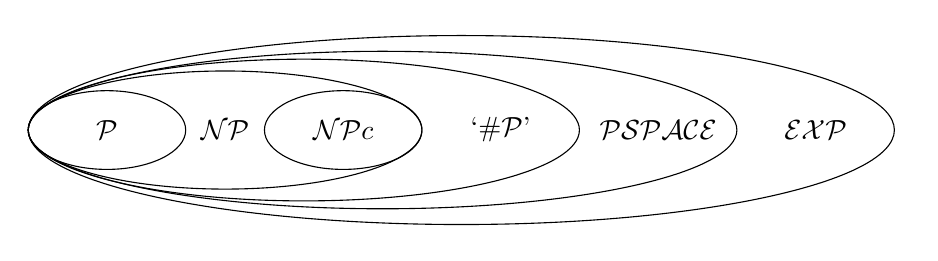
\begin{tikzpicture}
    \path (4.6,0) ellipse (5.6 and 1.3);
    \draw<1-> (0,0) ellipse (1 and .5);
    \node<1-> at (0,0) {$\p$};
    \draw<4-> (3.5,0) ellipse (4.5 and 1);
    \node<4-> at (7,0) {$\pspace$};
    \draw<3-> (1.5,0) ellipse (2.5 and .75);
    \node<3-> at (1.5,0) {$\np$};
    \draw<5-> (3,0) ellipse (1 and .5);
    \node<5-> at (3,0) {$\npc$};
    \draw<6-> (2.5,0) ellipse (3.5 and .9);
    \node<6-> at (5,0) {\lq$\sharpp$\rq};
    \draw<2-> (4.5,0) ellipse (5.5 and 1.2);
    \node<2-> at (9,0) {$\eXp$};
   \end{tikzpicture}
  \end{frame}
\subsection{Analytic Functions}
\begin{frame}
\frametitle{Data-types for functions}
We want to implement a data-type for functions and perform operations on this type.
\pause
\begin{fact}
For general polynomial time computable functions, many important operators have been shown to be computationally hard.\\
For example
\pause
\begin{itemize}[<+->]
\item Polynomial time computable functions may have noncomputable derivatives. (Ko 1983)
\item Parametric maximization is NP-hard. (Ko/Friedman (1982))
\item Integration is \#P-hard. (Friedman (1984))
\end{itemize}
\end{fact}
\end{frame}
\begin{frame}
\frametitle{Analytic Function}
An analytic function is a function locally given by a complex power series.\\
\begin{definition}[Analytic Function]
% \begin{columns}
% \begin{column}{0.4\linewidth}
$f : D \to \C $, $D \subseteq \C$ is analytic if for any $x_0 \in D$ the Taylor-series
$$ T(x) := \sum^\infty_{n=0} a_n(x-x_0)^n$$
converges to $f(x)$ for $x$ in a neighborhood of $x_0$.  
\end{definition}
\end{frame}
\begin{frame}
\frametitle{Some non-uniform results}

$$a_m =\frac{f^{(m)}(x_0)}{m!} 
, \,\, f(x) = \sum_{m=0}^\infty a_m(x-x_0)^k \,\ \text{ for } x \in B(x_0,R)
$$
\vfill
\begin{theorem}[Pour-El, Richards, Ko, Friedman, M\"uller (1987/1989)]
$f$ is (polytime) computable iff $(a_m)_{m \in \N}$ is.
\end{theorem}
 \onslide<2->{
From that polynomial time computability of the derivative and the anti-derivative of a function follows immediately.
}
\end{frame}
\begin{frame}
\frametitle{Some non-uniform results}
$$a_m =\frac{f^{(m)}(0)}{m!} 
, \,\, f(x) = \sum_{m=0}^\infty a_mx^k \,\ \text{ for } x \in B(0,R)
$$
\vfill
\begin{theorem}[M\"uller (1995)]
\begin{itemize}
\item The operator $f \to (a_m)_{m \in \N}$ is not computable.
\item The evaluation operator $((a_m)_{m \in \N},x) \to f(x) $ is not computable.
\end{itemize}
\end{theorem}
\pause
However, if we supply some additional (discrete) information those operators become computable.
\end{frame}
\subsection{Representing power series}
\begin{frame}
\frametitle{A practical representation for power series}
\begin{lemma}
  Let $f : \overline B(0,1) \to \R$ be real analytic and $(a_n)_{n \in \N}$ its power series around $0$.\\
  Then there exists an $k,A \in \N$ such that 
  \begin{enumerate}
  \item $\sqrt[k]{2}$ is a lower bound on the radius of convergence
  \item $\abs{a_n} \leq A \cdot 2^{-\frac{n}{k}}$
  \end{enumerate}
\end{lemma}
\pause
$A$ and $k$ can be used to make a tail estimate on
$$ \left | \sum_{n \geq N} a_n z^n \right |  $$
\end{frame}
\begin{frame}
\frametitle{Analytic Functions and Computational Complexity}
\begin{theorem}[Kawamura, R\"osnick, M\"uller, Ziegler (2013)]
  The following operators are computable in time polynomial in $n+k+\log(A)$, where $2^{-n}$ is the output precision.
\begin{enumerate}
\item evaluation
\item addition and multiplication
\item differentiation and anti-differentiation
\item parametric maximization
\end{enumerate}
\end{theorem}
\end{frame}
\section{Differential Equations}
\subsection{IVP Solving}
\begin{frame}
  \frametitle{Ordinary Differential Equations}
  We are further interested in the following problem:\newline
Consider Systems of Ordinary Differential Equations of the form
\begin{eqnarray*}
  \dot y_v(t) &=& F_v(t, y_1(t), \dots, y_t(t)) \\
  y_v(0) &=& 0 
\end{eqnarray*}
for $v=1,\dots,d$ and $F_v : \RR^{d+1} \to \RR$.
  \end{frame}
\begin{frame}
\frametitle{Complexity of Ordinary Differential Equations}
\begin{theorem}[Kawamura, 2010]
Consider the IVP
$$
y'(t)=f(t,y(t)) \quad;\quad y(0)=0.
$$
\pause
There exist functions $f: [0,1] \times [-1,1] \to \RR$ and $y: [0,1] \to [-1,1]$
such that $f$ is computable in polynomial time and Lipschitz continuous
but $y$ is PSPACE-hard.
\end{theorem}
The problem can be solved in PSPACE by applying the Euler method. (Ko)
\end{frame}
\begin{frame}
  \frametitle{Ordinary Differential Equations}
  We are further interested in the following problem:\newline
Consider Systems of Ordinary Differential Equations of the form
\begin{eqnarray*}
  \dot y_v(t) &=& F_v(t, y_1(t), \dots, y_t(t)) \\
  y_v(0) &=& 0 
\end{eqnarray*}
for $v=1,\dots,d$ and $F_v : \RR^{d+1} \to \RR$.
\pause
This is hard in the general case.
\pause
But if all $F_v$ are analytic, the solutions $y_v$ will again be analytic and the coefficients of the power series
can be computed in polynomial time if the $F_v$ are polynomial time computable.
  \end{frame}
\begin{frame}
  \frametitle{Multi-Dimensional Functions}
  Consider functions $f: \RR^d \to \RR$ complex analytic in a neighborhood of $0 \in \C^d$.
  \pause
  Their power series is given by
  $$\sum_{n_1, \dots, n_d \in \N} a_{n_1,\dots,n_d}x_1^{ n_1 } \dots x_d^{ n_d }$$
  \pause
  The beforementioned representation can be generalized.\\
  The main idea is let
  $$f(x_1, \dots, x_d) = \sum_{i \in \N} b_i\cdot x^i$$
  with
  $$b_{i} := \sum_{i_2, \dots, i_d \in \N^{d-1}} a_{i, \dots, i_d} \cdot x_2^{i_2} \dots x_d^{i_d}$$
  \pause
  $b_i$ can be evaluated by evaluating a $d-1$ dimensional analytic function.
%%   \begin{itemize}
%%   \item The beforementioned representation can be generalized for the multi-dimensional case
%%     \item Let $B$ and $q_i$ s.t. 
%% $ \abs{a_{i_1, \dots, i_d}} \leq \frac{B}{q_1^{i_1} \dots q_d^{i_d}} $
%%     \item Let $b_{i_1} := \sum_{i_2, \dots, i_d \in \N^{d-1}} a_{i_1, \dots, i_d} \cdot x_2^{i_2} \dots x_d^{i_d}$.
%%     \item Then $f(x_1, \dots, x_d) = \sum_{i \in \N} b_i\cdot x^i$
%% \item $\abs{b_i} \leq \frac{B}{q_1^i \cdot (1-\frac{x_2}{q_1}) \dots (1-\frac{x_d}{q_d})}$
%%   \item $b_i$ can be computed by evaluating a $d-1$ dimensional analytic function
%%   \end{itemize}
  \end{frame}
\section{Implementation}
\subsection{Implementation Details}
\begin{frame}
  \frametitle{DAG approach}
  \begin{center}
        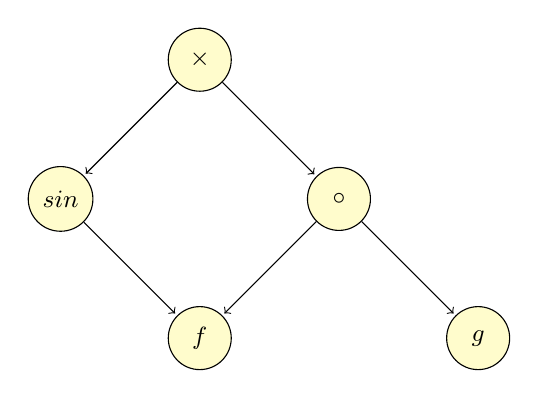
\begin{tikzpicture}[remember picture 
            ,->,shorten >=1pt,auto,node distance=2.5cm,minimum
              size=0.8cm,main node/.style={circle,fill=yellow!20,draw,font=\sffamily\small}]
    
    \node[main node] (1) {$\times$};
    \node[main node] (2) [below left of=1] {$sin$};
    \node[main node] (3) [below right of=1] {$\circ$};
    \node[main node] (4) [below left of=3] {$f$};
    \node[main node] (5) [below right of=3] {$g$};

    \path[every node/.style={font=\sffamily\small}]
    (1) edge (2)
    (2) edge (4)
    (1) edge (3)
    (3) edge (4)
    (3) edge (5);
  \end{tikzpicture}
  \end{center}
        \vfill
  Such a DAG can be evaluated or transformed to an analytic function.
\end{frame}
\begin{frame}
  \frametitle{Implementation}
  \foreach \x in {1,...,8} {
    \only<\x>{
      \includegraphics[width=1.1\textwidth]{class_overview\x}
    }
  }
\end{frame}
\begin{frame}
  \frametitle{ODE solving}
 Additionally there is an operator \code{solve\_ivp} for initial value problems of the form 
\begin{eqnarray*}
  \dot y_v(t) &=& F_v(t, y_1(t), \dots, y_t(t)) \\
  y_v(0) &=& 0 \text{ for }v=1,\dots,d
\end{eqnarray*}
\pause
The solution has parameters
$r' = \min(r, \frac{r}{M})$ 
$M' = r$ \newline
\pause
For initial values different from $0$ first use analytic continuation.
  \end{frame}
\begin{frame}
  \frametitle{Increasing the radius}
  \begin{itemize}
  \item Usually radius of the solution function will get very small
  \item One can use analytic continuation on the original function
  \item Compute $y_1 = y(t')$ for some small enough $t'$
  \item Solve the ODE $\dot y(t) = F(t, y(t))$; $y(t') = y_1$ 
  \end{itemize}
  \end{frame}
\begin{frame}
  \frametitle{Conclusion}
  \begin{itemize}
  \item Presented a data-type for multi dimensional analytic functions
  \item Several operators implemented
  \item Experiments show that from dimension $4$ operations on the power series become quite slow
  \item Can also solve systems of ordinary differential equations with the right hand side functions given by the type
  \item Radius of solution will usually get small so that many steps are needed
  \item Specialized functions for different types of ODEs?
  \item Parallelization
  \end{itemize}
  \end{frame}
%{
%\makeatletter % to change template
%    \setbeamertemplate{headline}[default] 
%    \def\beamer@entrycode{\vspace*{-\headheight}} 
%\makeatother
%\begin{frame}{References}
%\fontsize{6pt}{7.2}\selectfont 
%\nocite{*}
%\def\newblock{}
%\bibliographystyle{abbrv}

%\begin{thebibliography}{10}   
%
%  \beamertemplatearticlebibitems
%  \bibitem{6}
%	Harvey Friedman,
%    \newblock \emph{ The computational complexity of maximization and integration}, Adv. in Math. 53 (1984), no. 1, 80-98. MR 748898 (86c:03037)
%  \beamertemplatearticlebibitems
%  \bibitem{1}
%	Akitoshi Kawamura, Norbert Th. M\"{u}ller, Carsten R\"{o}snick, and
%Martin Ziegler
%    \newblock \emph{Parameterized Uniform Complexity in Numerics:
%from Smooth to Analytic, from NP-hard to Polytime}, pre-print (2012).
%
%  \beamertemplatearticlebibitems
%  \bibitem{7}
%	Ker-I Ko,
%    \newblock \emph{ Complexity theory of real functions}, Progress in Theoretical Computer Science, Birkh\"{a}user Boston Inc., Boston, MA, 1991.
%MR 1137517 (93i:03057)
%
%  \beamertemplatearticlebibitems
%  \bibitem{8}
%	Ker-I Ko,
%    \newblock \emph{  On the Computational Complexity of Ordinary Differential Equations}, Information and Control 58(1-3): 157-194 (1983)
%
%
%  \beamertemplatearticlebibitems
%  \bibitem{2}
%	Norbert Th. M\"{u}ller,
%    \newblock \emph{ The \irram: Exact Real Arithmetic in C++}, Computability and Complexity in Analysis (2000) .
%
%  \beamertemplatearticlebibitems
%  \bibitem{Mul95}
%	Norbert Th. M\"{u}ller,
%    \newblock \emph{ Constructive aspects of analytic functions}, Computability
%and Complexity in Analysis (Ker-I Ko and Klaus Weihrauch, eds.),
%Informatik Berichte, vol. 190, FernUniversit\"{a}t Hagen, September
%1995, CCA Workshop, Hagen, August 19-20, 1995, pp. 105-114.
%
%  \beamertemplatearticlebibitems
%  \bibitem{4}
%	Norbert Th. M\"{u}ller,
%    \newblock \emph{ Uniform Computational Complexity of Taylor Series}, ICALP 1987: 435-444
%
%  \beamertemplatearticlebibitems
%  \bibitem{5}
%	Norbert Th. M\"{u}ller,
%    \newblock \emph{ Polynomial Time Computation of Taylor Series}, Proc. 22 JAIIO - PANEL 1993
%
%  \beamertemplatearticlebibitems
%  \bibitem{9}
%	Marian B. Pour-El and J. Ian Richards,
%    \newblock \emph{ Computability in analysis
%and physics}, Perspectives in Mathematical Logic, Springer-Verlag,
%Berlin, 1989. MR 1005942 (90k:03062)
%  \beamertemplatearticlebibitems
%  \bibitem{11}
%	Florian Steinberg,
%    \newblock \emph{A type of Taylor series for the C++ library iRRAM for exact real arithmetic} (draft) last edited November 28, 2013
%  \beamertemplatearticlebibitems
%  \bibitem{10}
%	Klaus Weihrauch,
%    \newblock \emph{Computable analysis}, Texts in Theoretical Computer
%Science. An EATCS Series, Springer-Verlag, Berlin, 2000, An
%introduction. MR 1795407 (2002b:03129)
%
%  \end{thebibliography}

%\end{frame}
%}
\end{document}
